\part{Manejo y comunicación entre procesos}
\section{Procesos y API}
\paragraph{Proceso:} Es un programa en ejecución y todas las estructuras que debe mantener el sistema para su correcto funcionamiento. Entre ellas, los valores de los registros, el program counter, el stack del proceso, el área de memoria en la que se cargan las instrucciónes a  ejecutar (el programa propiamente dicho), el área de datos (contiene variables globales) y un heap de memoria (que es donde reserva memoria dinámica).

\subsection{Process Control Block (PCB)}\label{process::pcb}
Cada proceso está representado, en el sistema operativo, por un Process Control Block o Task Control Block. El mismo contiene información asociada a cada proceso, entre ellas:
\begin{itemize}
    \item El estado del proceso
    \item El program counter (la dirección de memoría de la próxima instrucción a ser ejecutada)
    \item Los registros del CPU,
    \item Información de Scheduling, como puede ser prioridad de ejecución
    \item Información de manejo de memoria, como las direcciones de los directorios de paginas o las tablas de segmentación. Y donde empiezan o termina cada una de sus partes (por lo gral, el proceso ve esto como una pila en la que se almacena el codigo. los datos, el heap y el stack del mismo).
    \item Estadísticas de uso del sistema
    \item Información de E/S (que dispositivos está usando, lista de archivos abiertos, etc)
\end{itemize}

El sistema mantiene una lista de todos los PCB de los procesos en ejecución que usa para tomar decisiones de schedulling.

\begin{figure}
    \begin{center}
        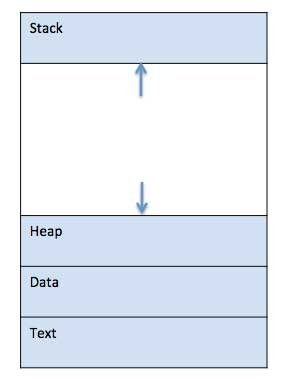
\includegraphics[width=0.25\textwidth]{imagenes/process_components.jpg}	
    \end{center}
    
    \caption*{Memoria de un proceso}
    \end{figure}

\subsection{Creación y control de un proceso}
\subsubsection{Creación de un proceso}

Durante su ejecución, un proceso puede crear nuevos procesos. En este caso llamamos \textbf{proceso padre} al proceso que crea nuevos procesos y \textbf{procesos hijos} a los procesos creados. Además, cada proceso hijo podrá crear otros procesos, formando así un \textbf{árbol} de procesos.

En la mayoría de los sistemas operativos, se asigna a cada proceso un identificador numérico único llamado \textbf{process id} o \textbf{pid} que sirve como índice para poder acceder a varios de sus atributos.

El nuevo proceso hijo creado necesitara de ciertos recursos para poder llevar a cabo su objetivo. Estos recursos podrán ser obtenidos directamente del sistema operativo o estar restringidos a los recursos del proceso padre.

En concreto, cuando el proceso padre decide crear un hijo, el sistema operativo hace una copia del PCB del padre con un nuevo PID. Ambos procesos comparten la tabla de páginas hasta que el proceso hijo necesite modificarlas. En este caso, cuando el hijo intenta usar alguna se genera un page fault (Ver sección \ref{page-fault}).

Cuando un proceso crea un nuevo proceso (\texttt{fork()}) hay dos posibilidades:

\begin{itemize}
    \item El padre y su hijo continúan ejecutando concurrentemente.
    \item El padre espera a que alguno o todos sus hijos terminen para seguir ejecutando (\texttt{wait()}).
\end{itemize}

Además, el nuevo proceso puede ser un duplicado de su padre o cargar un nuevo programa (\texttt{exec()})

\begin{center}
    \includegraphics[width=0.9\textwidth]{imagenes/process_creation.png}
    \end{center}

\subsubsection{Terminación}
Un proceso termina cuando ejecuta su última instrucción y pide al sistema operativo que lo borre usando la syscall \texttt{exit()}. En este momento, el proceso envía el código de estado con el que terminó a su padre y el sistema operativo libera todo los recursos que le había asignado.

La terminación puede ocurrir por varios motivos. Un proceso puede causar la terminación de otro usando las syscalls adecuadas (usualmente, esto puede hacerlo solo el proceso padre).

\subsubsection{Un poco más sobre las syscalls mencionadas}
\begin{itemize}
    \item \texttt{pid\_t fork()}: Crea un nuevo proceso. En el caso del creador se retorna el PID del hijo. En el caso del hijo, retorna 0.
    \item \texttt{int\ execve(const char* filename, char* const argv[], char* const envp[] )}: \\ Sustituye la imagen de memoria del programa por la del programa ubicado en filename.
    \item \texttt{pid\_t forkv()}: Crea un hijo sin copiar la memoria del padre, el hijo tiene que hacer \texttt{exec}.

    Un proceso creado con esta syscall comienza con sus páginas de memoria apuntando a las mismas que las de su padre. Recién cuando alguno escriba en memoria, se hace la copia. Esto se llama \textbf{Copy-On-Write}.

    \item \texttt{pid\_t wait(int* status)}: Bloquea al padre hasta que algún hijo termine o hasta que alcance el status indicado.
    \item \texttt{pid\_t waitpid(pid\_t pid, int* status)}: Igual al anterior pero espera a que el hijo con PID \texttt{pid} llegue a ese status.
    \item \texttt{void exit(int status)}: Finaliza el proceso actual.
    \item \texttt{clone(...)}: Crea un nuevo proceso. El hijo comparte parte del contexto con el padre. Es usado en la implementación de threads.
\end{itemize}

\paragraph{Fork Bomb:} Un proceso crea infinitos hijos.
\subsection{Estados de un proceso}\label{procesos::estados}
Durante su ejecución, un proceso va modificando su estado acorde al siguiente diagrama:

\begin{center}
    \vspace*{0.5cm}
    \includegraphics[width=0.9\textwidth]{imagenes/estados-proceso.png}
\end{center}

\begin{itemize}
    \item \textbf{Nuevo (New):} El proceso se está creando.
    \item \textbf{Listo (Ready):} El proceso está listo para ser ejecutado.
    \item \textbf{Bloqueado (Waiting):} El proceso está esperando a que ocurra algo (por ejemplo a que se complete una operación de entrada salida)
    \item \textbf{Ejecutando (Running):} El proceso se está ejecutando.
    \item \textbf{Terminado (Terminated):} El procesó termino de ejecutarse.
\end{itemize}

Es importante notar que solo un proceso puede estar \textbf{ejecutando} en un instante de tiempo de dado. Sin embargo, muchos procesos pueden estar bloqueados o listos simultáneamente.

\subsection{Scheduler}
\paragraph{Multiprocesador:} Un equipo con más de un procesador.
\paragraph{Multiprogramación:} La capacidad de un SO de tener varios procesos en ejecución.
\paragraph{Multiprocesamiento:} Se refiere al tipo de procesamiento que sucede en los multiprocesadores.
\paragraph{Multitarea:} Es una forma especial de multiprogramación, donde la conmutación entre procesos se hace de manera tan rápida que da la sensación de que varios programas están corriendo en simultáneo.
\paragraph{Multithreaded:} Son procesos en los cuales hay varios \textit{mini procesos} corriendo en paralelo (de manera real o ficticia).

\paragraph{Thread:} Son la unidad básica de utilización de la CPU, comprende un Thread ID, un contador de programa, un conjunot de registros y una pila. Los threads de un mismo proceso comparten la sección de datos y otros recursos del sistema operativo (como archivos abiertos y las señales que usan para comunicarse entre si). Un proceso con más de un thread mantiene una lista de los Thread Id en su PCB.
\subsubsection{Context Switching}
Una interrupción hace que el sistema operativo cambie la tarea de una CPU y corra un rutina del kernel. Cuando esto ocurre, el sistema, debe guardar el \textbf{contexto} del proceso que se está ejecutando para poder retornar a la ejecución del mismo cuando termine de atenderla. Este contexto es el PCB del proceso.

\vspace*{0.5cm}
\begin{center}
    \includegraphics[width=0.625\textwidth]{imagenes/context-switch.png}

\end{center}

    \subsubsection{Colas de procesos}
Una de las características de los sistemas operativos actuales es que nos permiten correr varias aplicaciones a la vez, sin embargo solo un proceso puede estar ejecutando en la CPU. Para darnos la sensación de simultaneidad, el SO hace lo que se llama \textbf{preemption}.

\paragraph{Preemption:} A cada proceso le asigna un \textbf{quantum} o una cantidad de tiempo durante la cual es ejecutado. Una vez que transcurrido ese tiempo, se guarda el contexto del proceso en memoria y se carga el contexto del próximo proceso a ejecutar.

El objetivo de la multiprogramación es intercambiar las tareas que se ejecutan en la CPU lo suficientemente rápido como para que el usuario pueda interactuar con dada programa como si estuviesen ejecutándose simultáneamente.Para esto existe un proceso especial llamado \textbf{Scheduler} que selecciona el próximo proceso que debe ser ejecutado.

El mismo dispone de varias colas de procesos en los que se encuentran los PCB de los procesos en ejecución. Los PCB se van encolando y desencolando de cada cola dependiendo del estado de cada proceso.

\vspace*{0.5cm}
\begin{center}
    \includegraphics[width=0.8\textwidth]{imagenes/process_queues.png}
\end{center}

Hay que tener en cuenta que para que sea posible realizar el cambio de contexto en cualquier momento, la función que debe estar ejecutando el proceso debe ser una función \textbf{reentrante}. Es decir, una funci[on que pueda ser interrumpida por el sistema operativo y que luego se pueda volver a llamar de forma segura desde donde se pausó su ejecución sin generar ningún problema. 

\subsection{Inter Process Communication (IPC)}
Los procesos que se están ejecutando concurrentemente en el sistema operativa pueden ser \textbf{procesos independientes} o \textbf{cooperativos}.

\paragraph{Procesos independiente:} Es un proceso que no puede afectar o ser afectado por otros procesos ejecuntandose en el sistema operativo.

\paragraph{Procesos cooperativos:} Son procesos que no son independientes (pueden afectar o ser afectados por otros procesos).

Los procesos cooperativos requieren de un mecanismo de comunicación que les permita intercambiar datos e información. Hay dos modelos fundamentales para hacer esto: \textbf{memoria compartida} y \textbf{Pasaje de mensajes}.

En el modelo de memoria compartida, se establece un área de memoría que es compartida entre procesos. Los procesos pueden intercambiar información leyendo y escribiendo en este área.

En el modelo de pasaje de mensajes, la comunicación se realiza a través de mensajes entre los procesos cooperativos.

\subsubsection{Pasaje de mensaje}
Los mensajes proveen a los procesos un mecanismo que permite que los procesos se comuniquen entre si y sincronicen sus acciones. Un sistema que permite el pasaje de mensajes provee al menos dos operaciones:
\begin{center}
    \texttt{send(message)}\hspace*{1cm}\texttt{receive(message)}
\end{center}

Los mensajes pueden tener una longitud fija o variable. La primera opción es más fácil de implementar pero hace que la programación de tareas sea mas tediosa. Los mensajes de longitud variable necesitan un sistema más complejo pero permite más agilidad a la hora de programar tareas.

Si un proceso $P$ y $Q$ se quieren comunicar, entonces debe existir un \textbf{link de comunicación} entre ellos. Para crear este link, se deben tener en cuenta el tipo de comunicación que se desea ofrecer:
\begin{itemize}
    \item \textbf{Direccionamiento}
    \begin{itemize}
        \item \textbf{Conexión directa:} Cada proceso debe explicitar el nombre del proceso destinatario/receptor:
        \begin{itemize}
            \item \texttt{send(P, message)} - Envía un mensaje al proceso $P$
            \item \texttt{receive(Q, message)} - Recibe un mensaje del proceso $Q$
        \end{itemize}

        En este caso, el link de comunicación se establece automáticamente entre cada par de procesos que quiere comunicarse. Y cada proceso sabe la identidad del otro.

        \item \textbf{Comunicación indirecta:} Los mensajes son enviados a buzones (\textbf{mailboxes}) o puertos (\textbf{ports}). Cada buzón tiene un identificador único. Un proceso puede comunicarse con otro a través de varios buzones.
        \begin{itemize}
            \item \texttt{send(A, message)} - Envía un mensaje al buzón $A$
            \item \texttt{receive(A, message)} - Recibe un mensaje del buzón $A$
        \end{itemize}

        En este esquema, un link se establece entre dos procesos solo si comparten un buzón. Además un link puede estar asociado a varios pares de procesos e incluso puede haber varios links entre dos mismos procesos.

    \end{itemize}
    \item \textbf{Sincronización:} El pasaje de mensajes puede ser bloqueante (síncrono) o no bloqueante (asíncrono):
    \begin{itemize}
        \item \textbf{Envío bloqueante:} El proceso que envía un mensaje espera a que el mismo sea recibido por su destinatario.
        \item \textbf{Envío no bloqueante:} El proceso envía el mensaje y sigue su ejecución.
        \item \textbf{Recepción bloqueante:} El proceso se bloquea hasta que recibe un mensaje.
        \item\textbf{Recepción no bloqueante:} El receptor recibe un mensaje válido o null.
    \end{itemize}
    \item \textbf{Buffering}: Los mensajes intercambiados entre procesos deben almacenarse en una cola temporal. Estas colas pueden ser de tres tipo:
    \begin{itemize}
        \item\textbf{Capacidad Cero:} El link no puede tener mensajes en espera. El remitente debe bloquearse hasta que el mensaje sea recibido.
        \item \textbf{Capacidad acotada:} La cola tiene una capacidad finita $n$ por lo que puede haber a lo sumo $n$ en espera. Si la cola no está llena se puede enviar un mensaje, sino el remitente debe bloquearse hasta que se que haya espacio disponible.
        \item \textbf{Capacidad infinita:} El remitente nunca se bloquea.
    \end{itemize}
\end{itemize}

\subsubsection{Sockets}
Los sockets son los extremos de una comunicación que usan dos procesos para comunicarse a través de una red. Cada socket está identificado por una dirección IP y un número de puerto. 	

En general, en este tipo de links, se usa una arquitecutra cliente-servidor: El servidor espera a que un cliente haga un pedido y, una vez que lo recibe, acepta la conexión del socket del cliente para completar la conexión. El número del socket del servidor, en general, va a ser menor o igual a 1024. Estos puerstos son los puertos conocidos (\textit{well known ports}) e implementan distintos protocolos estandarizados.

Cuando el proceso cliente inicia la conexión, la computadora que lo está ejecutando le asigna un puerto arbitrario cuyo número es mayor a 1024.
\subsubsection{Pipes}
Un \textbf{pipe} es un canal que provee una de las formas más simples de comunicación entre dos procesos aunque tienen sus limitaciones. Al implementar un pipe, se debe tener ciertas consideraciones: 
\begin{enumerate}
    \item ¿El pipe permite comunicación bidireccional o unidireccional?
    \item Si es bidireccional, es \textbf{half-duplex} (para mandar información se debe esperar a que el otro extremo del pipe termina de hacerlo) o \textbf{full-duplex} (la información puede viajar de un lado a otro y viceversa simultaneamente).
    \item ¿Debe existir alguna relación entre los procesos que se están comunicando (por ejemplo, padre-hijo)?
    \item ¿Los procesos se van a poder comunicar dentro de una red o tienen que estar en la misma maquina?
\end{enumerate}

\paragraph{Ordinary pipes:} Permiten que dos procesos se comuniquen en modo productor-consumidor: El productor escribe en un extremo del pipe (extremo de escritura) y el consumidor lee desde el otro extremo (extremo de lectura). Estos pipes son unidireccionales. Si se necesita una comunicación bidireccional se debe crear otro pipe que permita mandar datos en la otra dirección.

Este tipo de pipes requieren que los procesos que se comunican tengan una relación padre-hijo y dejan de existir una vez que la comunicación termina.

\paragraph{Named pipes:} Proveen comunicación bidireccional y no necesitan que los procesos estén relacionados. Una vez que es establecido, varios procesos pueden usarlo para comunicarse y continuan existiendo incluso después de que las comunicaciones hayan finalizado.

\subsection{E/S bloqueante / no bloqueante}
    Cuando un proceso necesita escribir o leer información de algún dispositivo necesita realizar operaciones de \textbf{entrada/salida}

    Estas operaciones son muy lentas por lo que quedarse bloqueado es un desperdicio de tiempo.

    \paragraph{Busy Waiting:} El proceso no hace nada pero no libera el CPU. Se gastan ciclos de procesamiento en hacer nada.

    Para evitar esto se utilizan algunas técnicas que permiten al SO seguir ejecutando mientras espera la respuesta de los dispositivos:

    \begin{itemize}
        \item \textbf{Polling}: El proceso libera la CPU pero todavía recibe un quantum cada tanto que desperdicia hasta que la E/S esté terminada.
        \item \textbf{Interrupciones:} Esto permite la multiprogramación. El SO no le otorgá más quantum al proceso hasta que su E/S esté lista. El hardware comunica esto mediante una interrupción que hace que el proceso se despierte.
    \end{itemize}

    \subsection{Manejo básico de un shell Unix}
\subsubsection{File descriptors:}
    En Unix, cada proceso se crea con una tabla que le permite identificar cuales son los archivos que tiene abiertos. Cada índice es un \textbf{file descriptors} que usa el Kernel para saber como leer/escribir datos en los distintos archivos (en Unix, el teclado y la pantalla se modelan como archivos).
    
    Además, cada proceso hereda de su proceso padre tres archivos abiertos que ocupan los file descriptors 0, 1 y 2 y representan la entrada estándar (\textbf{stdin}), la salida estandar (\textbf{stdout}) y el error estandar (\textbf{stderr}), respectivamente.
    
    Linux provee de dos llamadas al sistema que nos permiten leer/escribir a un archivo usando su file descriptor \texttt{fd}:
    
    \begin{center}
        \texttt{ssize\_t read(int fd, void *buf, size\_t count)}

        \texttt{ssize\_t write(int fd, const void *buf, size\_t count);}
    \end{center}
    
Aquí \texttt{buf} es un puntero a donde se almacenan los datos a leer o escribir y \texttt{count} la cantidad de bytes que hay escribir/leer.

\subsubsection{Comandos de consola}
\begin{itemize}
    \item \texttt{echo} escribe lo que le pasemos como parámetro en su \textbf{stdout}.
    \begin{center}
        \texttt{echo ``Esto es un mensaj''}	\end{center}
    \item \texttt{>} Se le indica a la consola que el \textbf{stdout} se redirija a un archivo:
    \begin{center}
        \texttt{echo ``Esto es un mensaje'' > mensaje.txt}
    \end{center}
    \item \texttt{|} Redirige el \textbf{stdout} de un proceso hacia el \textbf{stdin} de otro:
    
    \begin{center}
        \texttt{echo ``Esto es un mensaje'' | wc -c}
    \end{center}

    En este caso, el primer proceso ejecuta el comando \texttt{echo} que imprime en \textbf{stdout} el mensaje \texttt{``Esto es un mensaje''}. El segundo proceso recibe por \textbf{stdin} lo que se escribió en el \textbf{stdout} del proceso que ejecutó \texttt{echo}
\end{itemize}
\printbibliography[keyword=procesos,title=Bibliografía]

\newpage
    
\section{Scheduling} 
    En sistemas con un único procesador, solo se puede correr de a un proceso por vez. Uno de los objetivos de la multiprogramación es que todo el tiempo se esté ejecutando un proceso para maximizar el uso de CPU.
    
    Cada vez que el CPU entra en estado IDLE, el sistema debe seleccionar alguno de los procesos que estén listos para ser ejecutados. El proceso de selección es llevado a cabo por el \textbf{scheduler} usando la que se llama \textbf{cola de ejecución}.
    
    \subsection{Objetivos de la política de scheduling}
    Diferentes algoritmos de schedulling tienen diferentes propiedades y la elección de los mismos depende de las situación particular del sistema. Por lo general, un algoritmo de schedulling busca optimizar alguna combinación de las siguientes propiedades:
    
    \begin{itemize}
        \item \textbf{Eficiencia}: Maximizar la cantidad de tiempo que el CPU esté ocupado.
        \item \textbf{Rendimiento (Throughput)}: Maximizar el número de procesos terminados por unidad de tiempo.
        \item \textbf{Tiempo de ejecución (Turnaround time)}: Minimizar el tiempo total que le toma a un proceso ejecutar completamente (el intervalo de tiempo desde que el proceso se crea hasta que temina, incluye tiempo de esperas en la cola de procesos).
        \item \textbf{Ecuanimidad (Fairness)}: Que Cada proceso reciba una dosis ``justa" de CPU (para alguna definición de justicia).
        \item \textbf{Carga del sistema (Waiting time)}: Minimizar la cantidad de tiempo que un proceso esté en la cola de espera.
        \item \textbf{Tiempo de respuesta (Response time)}: Minimizar el tiempo de respuesta percibido por los usuarios interactivos.
        \item \textbf{Latencia}: Minimizar el tiempo requerido para que un proceso comienze a dar resultados.
        
        \item \textbf{Liberación de recursos:} Hacer que terminen cuanto antes los procesos que tiene reservados más recursos.
    \end{itemize}
    Muchos de estos objetivos son contradictorios. Si los usuarios del sistema son heterogéneos, pueden tener distintos intereses por lo que cada política de scheduling debe buscar maximizar una función objetivo que es una combinación de estas metas tratando de impactar lo menos posible en el resto.
    
    \subsection{Scheduling con y sin desalojo}
    
    El sistema puede tomar decisiones de scheduling en alguna de las siguientes situaciones:
    \begin{enumerate}
        \item Cuando un proceso pasa de estado \textit{Ejecutando} al estado de espera (por ejemplo cuando hace un request de entrada salida)
        \item Cuando pasa de \textit{Ejecutando} a \textit{Listo}
        \item Cuando pasa de \textit{Esperando} a \text{Listo}
        \item Cuando termina.
    \end{enumerate}
    
    \paragraph{Starvation (Bloqueo indefinido)}: Un proceso sufre de starvation cuando está listo para ser ejecutado pero la CPU nunca le asigna clocks de reloj en lo que ejecutar.
    
    \paragraph{Scheduling sin desalojo:} Tambien conocido como \textbf{coperativo} o \textbf{nonpremptive}, se da cuando las decisiones de scheduling solo toman lugar en las situaciones $1$ y $4$, es decir se espera a que el proceso haya terminado o esté inactivo. Tiene como desventaja que si un proceso muy largo toma control del procesador se puede generar un cuello de botella y otros procesos mas cortos tardarían demasiado en ser ejecutados.
    
    \paragraph{Scheduling con desalojo:} Tambien llamado scheduling \textit{apropiativo} o \textit{preempitve}, se vale de la interrupción del clock para decidir si el proceso actual debe seguir ejecutando o le toca a otro. No da garantías de continuidad a los procesos.
    
    Por lo general se usa una combinación de los dos tipos de scheduling para decidir las políticas adecuadas.

    \subsection{Políticas de scheduling}
    \subsubsection{First In/First Out (FIFO)}
    El algoritmo FIFO (también conocido como First Come, First Served) es una de las políticas de scheduling más simples. Los process control block (PCB) se ubican en una cola, el próximo proceso a ejecutar es el que está en la cabeza. Cuando un proceso está listo para ser ejecutado se lo encola al final.
    
    Por un lado, es simple de implementar. Por otro, el tiempo de espera promedio de un proceso es bastante largo y hay que tener en cuenta que es un algoritmo sin delajo. Si llega un proceso que requiera mucho tiempo de CPU, tapona todos los demás, esto se llama \textbf{convoy effect}.
    
    \subsubsection{Shortest Job First (SJF)}
    Este algoritmo asocia cada proceso con su duración y ejecuta primero aquellos que duran menos. Está ideado para sistemas donde predominan los trabajos batch y está orientado a maximizar el throughput.
    
    Si los procesos ejecutados tienen un comportamiento regular, se puede usa el historial de ejecución para predecir los tiempos ejecución de los procesos actuales. Sin embargo, en sistemas con procesos heterogéneos no es posible saber cuanto tiempo de ejecución va a necesitar cada uno por lo que no es posible implementar este algoritmo.
    
    \subsubsection{Round Robin}
    Este algoritmo está especialmente diseñado para sistemas de tiempo compartido (varios procesos deben usar el cpu al mismo tiempo). Se comporta de manera similar al FIFO, solo que se agrega desalojo para permitir al sistema ejecutar otros procesos.
    
    Para esto se define una pequeña unidad de tiempo llamada \textbf{quantum} durante la cual puede correr cada proceso. Si la ráfaga de procesamiento (CPU Burst) de un proceso es mas chico que el quantum, entonces el mismo la liberará y el scheduler eligirá el siguiente proceso a ejecutar.
    
    Si el CPU Burst toma más de un quantum, entonces se enviará una interrupción al sistema. Éste desalojará el proceso, cambiará el contexto y el proceso que se estaba ejecuntando se pondrá al final de la cola de ejecución.
    
    El rendimiento de este tipo de algoritmos depende del tamaño del quantum. Por un lado, si el quantum es demasiado largo, la política de Round Robind termina siendo una FIFO. Por el otro, si el quantum es extremadamente pequeño se pueden producir una gran cantidad de cambios de contexto, por lo que una gran parte del tiempo del CPU sería gastado solo en esto.
    
    En general, se debe elegir el quantum de tal manera que la mayoria de los procesos termine su CPU Burst durante el mismo pero no tan largo como para que sea un FIFO.
    
    \subsubsection{Multiples colas}
    Otra idea, es serparar los procesos en distintas colas de acuerdo a la duración de su CPU Burst. Cada cola tendrá mas prioridad sobre la otra. Si un proceso toma demasiado tiempo, entonces se lo mueve a una cola con una prioridad menor. 
    
    Este esquema, da mayor prioridad a los procesos interactivos y aquellos procesos que estén esperando demasiado tiempo pueden ser movidos a colas de mayor prioridad para evitar starvation.

\printbibliography[keyword=scheduling,title=Bibliografía]

\newpage
\section{Sincronización de procesos (Memoria compartida)}
Normalmente, los sistemas operativos tratan de prevenir que un proceso acceda a la memoria de otro. Sin embargo, si dos o mas procesos deciden remover esta restricción pueden definir una región de memoria mediante la cual podrán intercambiar información. En este caso, los mismos procesos son los responsables de asegurar que no escriben simultáneamente en esta región.

\paragraph{Contención y concurrencia:} Ocurre cuando uno o más procesos tratan de acceder al mismo recurso de manera simultánea. Esto puede causar que algunas secuencias de ejecución terminen con resultados erróneos.

\subsection{Modelo Productor-Consumidor}
Uno de los paradigmas clásicos de procesos cooperativos con este tipo de intercomunicación es el de \textbf{productor-consumidor}. En este esquema, un proceso \textbf{productor} debe producir información que va a ser consumida por un proceso \textbf{consumidor}.

Una posible implementación de este problema, es definir un buffer en una región de memoria compartida entre ambos procesos en la cual el productor pueda encolar elementos mientras que el consumidor los desencola. Ambos procesos deben estar sincronizados de tal manera que el consumidor no trate de desencolar elementos si la cola está vacía.

Se pueden consierar dos tipos de buffers en esta solución:
\begin{itemize}
    \item \textbf{Unbounded buffer} (buffer infinito): No posee límites de espacio. El consumidor tiene que esperar a que el buffer tenga algo y el productro siempre puede agregarle elementos.
    \item \textbf{Bounded buffer} (buffer limitado): Tiene un tamaño fijo. Si está vacío, el consumidor debe esperar a que haya algo. Si está lleno, el productor debe esperar a que se haya consumido por lo menos un elemento antes de agregar otro.
\end{itemize}

Veamos una solución con buffer limitado:

\vspace*{0.25cm}
\begin{center}
        \textbf{Zona de memoria compartida}
    \begin{minted}[tabsize=28]{cpp}
    buffer in[BUFFER_SIZE];
    int cant = 0;
    \end{minted}
\end{center}
\setlength{\columnseprule}{0.4pt}
\noindent\rule{\textwidth}{0.4pt}
\begin{multicols}{2}
    \begin{center}
    \textbf{Proceso productor}

    \begin{minted}[tabsize=2]{cpp}
    while(true){
        while(counter == BUFFER_SIZE) {};
        in.push(item);
        counter++;
    }
    \end{minted}
\columnbreak
\textbf{Proceso consumidor}
    \begin{minted}[tabsize=2]{cpp}
    while(true){
        while(counter == 0) {};
        item = pop(in);
        counter--;
    }
    \end{minted}
    \end{center}
\end{multicols}
\setlength{\columnseprule}{0pt}

\subsubsection{Condiciones de carrera (race conditions)}
En el ejemplo anterior, si bien el código para cada proceso puede parecer correcto, puede haber errores si ambos se ejecutan de manera concurrente. Supongamos que las lineas \mintinline{cpp}{counter++} y \mintinline{cpp}{counter--} tienen la siguiente forma en lenguaje maquina:
\begin{center}
    \begin{minipage}{0.8\textwidth}
\begin{multicols}{2}
    \noindent\mintinline{cpp}{counter++}:
    \begin{minted}{cpp}
        register1 = counter;
        register1 = register+1;
        counter = register1	
    \end{minted}
    
    \noindent\mintinline{cpp}{counter--}:
    \begin{minted}{cpp}
        register2 = counter;
        register2 = register2-1;
        counter = register2;
    \end{minted}
\end{multicols}
\end{minipage}

\end{center}

Supongamos que el valor inicial de \texttt{counter} es 5, el proceso productor agrega un elemento al buffer, el consumidor quita el primer elemento encolado y ambos procesos ejecutan \texttt{counter++} y \texttt{counter--} de manera concurrente, entonces una posible secuencia de ejecución de estas instrucciones podria ser:

%\vspace*{0.5cm}
\begin{center}
\begin{tabularx}{0.8\textwidth}{|L{1.3}|L{1.3}|C{0.4}|}
    \hline 
    \textbf{Productor} & \textbf{Consumidor} & \textbf{\texttt{counter}} \\
    \hline
    & & 5 \\
    \hline
    \texttt{register1 = counter} & & 5 \\
    \hline
    \texttt{register1 = register + 1} &  & 5 \\
    \hline
     & \texttt{register2 = counter}  & 5 \\
     \hline
     &  \texttt{register2 = register - 1} & 5 \\
      \hline
     \texttt{counter = register1} &  & 6 \\
       \hline
    & \texttt{counter = register2} & 4 \\
    \hline
    \end{tabularx}
\end{center}

En este caso, el consumidor comienza a modificar la variable \texttt{counter} antes de que el productor guarde el valor correspondiente en memoria y no se ``entera" que un nuevo elemento fue agregado a la cola (por lo que todavía habría 5 elementos en ella). Entonces se genera una inconsistencia entre el valor de \texttt{counter} y la cantidad elementos en el buffer.

Este tipo de situaciones se llama \textbf{race condition}: Se da cuando varios procesos pueden acceder y modificar la misma variable de manera concurrente y el valor final de ésta depende del orden particular en el que se hayan realizado los accesos a la misma.

\subsection{Secciones críticas}
La idea es que cada proceso que se esté ejecutando en el sistema tenga un segmento de código, llamado \textbf{sección crítica}, que solo se puede ejecutar cuando ningún otro proceso esté en ella. Es decir, no puede haber mas de un proceso ejecutando su sección crítica al mismo tiempo. Para poder implementar esto, por lo general, se divide el código del segmento en tres partes:
\begin{enumerate}
    \item \textbf{Entry section:} En donde el proceso pide permiso para acceder a la sección crítica.
    \item \textbf{Critical section:} La zona crítica per se, en la que se puede manejar la memoria compartida
    \item \textbf{Exit section:} Donde el proceso avisa al sistema que dejó de realizar operaciones críticas.
\end{enumerate}
\begin{figure}
    \centering
    \includegraphics[width=0.5\textwidth]{imagenes/structura-seccion-ciritca}
    \caption{Estructura general de un proceso que implementa sección crítica}
    \label{fig:structura-seccion-ciritca}
\end{figure}

Una buena implementación de esta método debe sastifacer los siguientes requerimientos:
\begin{enumerate}
    \item \textbf{Exclusión mutua}: Si un proceso está ejecutando su sección crítica,
     entonces ningún otro debe estar ejecutando la suya.
     \item \textbf{Progreso}: Si un proceso necesita entrar a su sección crítica, entonces se le dará permiso para hacerlo en algún momento.
    \item \textbf{Bounded waiting (espera acotada/no bloqueante	)}: Si un proceso $P$ pide entrar a la sección crítica, entonces hay un límite en la cantidad de veces que se le da mayor prioridad a otros procesos sobre $P$.
\end{enumerate}
\subsubsection{Instrucción TestAndSet}
Los sistemas opertivos modernos proveen una instrucción de hardware especial que nos permite testear y/o modificar una palabra de manera \textbf{atómica}, es decir como unidad no interrumpible de ejecución. Cuando se utiliza, el sistema no ejecuta ninguna otra instrucción hasta que ésta haya terminado. Para abstraernos, de sistemas operativos espécificos, llamemos esta instrucción \texttt{testAndSet()}, la misma toma como paramétro una variable booleana que se va a setear en \mintinline{cpp}{true} y va devolver el valor anterior:

\begin{center}
    \begin{minipage}{0.5\textwidth}
        \begin{minted}[tabsize=2]{cpp}
bool testAndSet(bool* source) {
    bool result = *source;
    *source = true;
    return result;
}
        \end{minted}
    \end{minipage}
\end{center}

En este caso, un sistema de procesos que utilice esta instrucción podría tener una variable booleana compartida llamada \textbf{lock} que controlaria el acceso a la secciónes criticas de cada proceso, si \mintinline{cpp}{lock == false} entonces es posible entrar, si es \mintinline{cpp}{true} el proceso debe esperar:

\begin{minted}[tabsize=2]{cpp}
        bool lock;
        
        void main() {
            while(true) {
                ...
                while(testAndSet(&lock)) {};
        
                /* Sección crítica */
        
                lock = false;
                ...
            }	
        }
\end{minted}

\subsubsection{Instrucción Test and Test an Set}
Es una pequeña mejora a Test and Set, en este caso, primero se realiza el chequeo si la variable esta seteada o no, una vez que la condicion deja de cumplirse se realiza el test and set. Esto nos permite mantener el busy waitint sin la necesidad de realizar la escritura que se produce cada vez que entramos a Test and Set:

\begin{center}
    \begin{minipage}{0.5\textwidth}
        \begin{minted}[tabsize=2]{cpp}
bool testAndSet(bool* source) {
    while(true) {
        while(test(source)) {}
        if(!testAndSet(source)) return;
    }
}
        \end{minted}
    \end{minipage}
\end{center}

\subsubsection{Instrucción CompareAndSwap}\label{compareAndSwap}
Es una instrucción primitiva ofrecida por varios porcesadores que toma 3 argumentos: una dirección de memoria, un valor esperado y un valor que se debe escribir en esa posición si se encuentra el valor esperado:

        \begin{minted}[tabsize=2]{cpp}
bool testAndSet(int* value, int expected, int new_value) {
    int temp = *value;
    if(*value == expected) *value = new_value
    return temp;
}
        \end{minted}

\subsubsection{Mutex Lock o SpinLock (busy waiting)} 
La solución basada en hardware presentada en la sección anterior, generalmente es inaccesible a los programadores. Por esta razón, los sistemas operativos diseñan herramientas básicas para implementar secciones críticas: La más simple de ellas es el \textbf{mutex lock}. El mismo contiene de una variable booleana \texttt{avaliable} que indica si el lock está disponible o no y provee dos funciones: 

\begin{itemize}
\item \texttt{acquire()}: Permite a un proceso adquirir el lock y bloquear otros procesos el acceso a su sección crítica. Si un proceso llama a esta función y el lock ya estaba tomado, el proceso queda en espera hasta que el lock se libere.

\begin{minted}[tabsize=2]{cpp}
    void aquire() {
        while(!avaliable) {}; // Busy wait
        avaliable = false;	
    }
\end{minted}
\item \texttt{release()}: Libera el lock para que los procesos bloqueados puedan continuar con su ejecución.
\begin{minted}[tabsize=2]{cpp}
    void release() {
        avaliable = true;	
    }
\end{minted}
\end{itemize}

Ambas funciones deben ejecutarse de manera atómica por lo que generalmente son implementadas usando la instrucción de hardware \texttt{testAndSet()}. La principal desventaja es que requiere de \textbf{busy waiting} (mientras un proceso está en su sección crítica, cualquier proceso que llame a \texttt{aquire()}) debe ciclar continuamente hasta que el lock se libere. Esto es un problema en los sistemas de multiprogramación, donde los ciclos de CPU son compartidos entre varios procesos.

Por lo general, se usan cuando las secciones críticas de los procesos no requieren de mucho uso de CPU y el recurso es liberado relativamente rápido (por ejemplo, si es una variable compartida entera).

\subsection{Semáforos}
Un semáforo \texttt{S} es una estructura que contiene una variable entera \texttt{value} y una lista \texttt{list} de procesos a las que se puede acceder mediante dos operaciones atómicas:
\begin{itemize}
    \item \texttt{wait()}: Cuando un proceso llama a esta operación, si \texttt{S.value} es negativo entonces debe esperar. Sin embargo, en vez de hacer busy waiting, el proceso se bloquea (entra en estado \texttt{waiting}, ver sección \ref{procesos::estados}) y se encola en \texttt{S.list}. Luego, el control es transferido al scheduler que selecciona otro proceso para ejecutar.
\begin{minted}[tabsize=2]{cpp}
    void wait(S) {
        S.value--;
        if(S.value < 0) {
            agregar este proceso a S.list;
            block();
        }
    }
\end{minted}
    \item \texttt{signal()}: Cuando un proceso termina de ejecutar su sección crítica, llama a esta operación que indica al semáforo que puede despertar alguno de los procesos en espera. Para esto, se quita algun proceso de la lista y se lo pasa a estado \texttt{ready} para que que el scheduler lo vuelva a tener en cuenta.
    \begin{minted}[tabsize=2]{cpp}
        void signal() {
            S.value++
            if(S.value <= 0) {
                quitar proceso P de S.list;
                wakeup(P);
            }	
        }
    \end{minted}
\end{itemize}

Este tipo de semáforos está pensado para administrar la asignación de recursos (de los cuales se tiene una o más instancias) del sistema.

La lista de procesos en espera puede ser implmentada por un campo \texttt{link} en cada process control block (sección \ref{process::pcb}) y la lista de procesos del semáforo en realidad es una lista punteros a PCBs.

Los semáforos se usan cuando realmente vale la pena realizar los context switch necesarios para que el sistema pueda avanzar. Por ejemplo, es deseabales utilizarlos en sistemas con único procesador donde el busy waiting solo desperdiciría ciclo de reloj (ya que el estado de la variable que se esta chequeando no va a ser cambiado dentro del mismo proceso)
%\paragraph{Estructura básica de un proceso con testAndSet()}: Dado un sistema compuesto de $n$ procesos, una posible implementación de secciones críticas que cumplan los tres requirimientos mencionados es la siguiente:
%
%\vspace*{0.25cm}
%\textbf{Zona de memoria compartida}
%	\begin{minted}[tabsize=2]{cpp}
%		buffer waiting[n] = { 0 }; // n = cantidad de procesos
%		bool lock = 0;
%		int  next_process = 0;
%	\end{minted}
%
%\textbf{Proceso número $i$:}
%\begin{minted}[tabsize=2]{cpp}
%		while(true){
%			...	
%			waiting[i] = true;
%
%			while(waiting[i] && testAndSet(&lock)) {}
%			waiting[i] = 0;
%			/* sección crítica */		
%			next_process = next(i);
%			lock = false;
%			...
%		}
%	\end{minted}
%
%Donde \texttt{next(i)} calcula cual es el índice del próximo proceso que debe entrar en la sección crítica de la siguiente forma:
%
%\begin{minted}[tabsize=2]{cpp}
%	int next(int actual_process) {
%		// Buscamos el proximo proceso que este esperando para entrar en 
%		// la sección crítica
%		next = (i + 1) % n;
%		while (next != actual && !waiting[next]) next = (next + 1) % n;
%	
%		// Si no encontré ninguno, entonces no hay nadie esperando 
%		// y libero el lock, sino le doy permiso a que ejecute la sección critica 
%		// al proceso que encontré
%		if(next == actual) lock = false;
%		else waiting[next] = false;
%	}
%\end{minted}

\subsubsection{Monitores y variables de condición}
Aunque los semáforos proveen un mecanismo conveniente y efectivo para realizar la sincronización de proceso, usarlos incorrectamente puede conllevar a errores dificiles de detectar, ya que estos pueden ocurrir en una secuencia de ejecución particular.

Para resolver estos errores, se dasorrollo un tipo abstracto de dato llamado \textbf{monitor} que contiene un conjunto de operaciones que ya aseguran mutual exclusion. El monitor declara variables locales que definen su estado junto con las funciones que operan esas variables (y son la única forma de accederlas).

\begin{minted}[tabsize=2]{cpp}
Monitor M {
/** Declaración de variables compartidas **/
var x;
var y;
var z;

/** operaciones sobre esas variables **/
function op1(...) { ... }
function op2(...) { ... }
function op3(...) { ... }
function constructor(...) { ... }
}
\end{minted}

La implementación del monitor debe asegurar que nunca hay más de un proceso activo dentro del mismo. De esta forma, el programador no debe preocuparse por los requerimientos de sincronización. Sin embargo, la construcción presentada no alcanza para modelar algunos mecanismos de sincronización, por lo que se agrega los mismos lo que se llama \textbf{variables de condición}.

La únicas operaciones invocadas en una variable de condición son \texttt{signal()} y \texttt{wait()}. \texttt{wait()} suspende el proceso hasta que otro proceso llame al \texttt{signal()}. Si no hay procesos esperando, entonces \texttt{signal()} no tiene efecto. Este tipo de variables se puede implementar con semáforos. 

Supongamos que definimos una variable de condición $c1$ sobre el monitor $M$ y que un proceso $P$ invoca $c1.signal()$. Si existe un proceso $Q$ suspendido asociado a $c1$ entonces $Q$ debería poder ingresar al monitor, sin embargo, $P$ sigue estando dentro del mismo. Tenemos dos posibilidades:

\begin{enumerate}
    \item \textbf{Signal and wait:} $P$ se pausa y espera a que $Q$ salga del monitor o espera a que se cumpla otra condición.
    \item \textbf{Signal and continue:} $Q$ espera a que $P$ deje el monitor o espera a que se cumpla otra condición.
\end{enumerate}

Por un lado, tiene sentido dejar que $P$ siga ejecutandose dentro del monitor. Por otro, si permitimos esto, puede llegar a pasar que para el momento en el que $Q$ sea activado, la condición lógica que estaba esperando deje de valer. En muchos casos, lo que se hace es hacer que la ultima instrucción que se ejecuta dentro del monitor sea un \texttt{signal()}. De esta manera, $P$ deja la sección crítica, puede seguir su ejecución y $Q$ puede entrar en su propia sección.

\subsubsection{Deadlock}
La implementación de semáforos puede resultar en una situación donde dos o más procesos se pueden quedar esperando por un evento que solo puede ser causado por otro proceso en espera.  Cuando esto sucede, se dice que estos procesos están en \textbf{deadlock}.

Decimos que un conjunto de procesos está en estado de deadlock cuando cada proceso del conjunto está esperando por un evento que solo puede ser causado por otro proceso de ese conjunto.

\paragraph{Ejemplo:} Supongamos que tenemos dos procesos $P_0$ y $P_1$ que hacen uso de los semáforos binarios $S$ y $Q$ y se produce la siguiente secuencia de comandos:

\begin{center}
\begin{tabularx}{0.8\textwidth}{|C{0.5}|C{0.5}|L{2}|}
    \hline 
    \textbf{$P_0$} & \textbf{$P_1$} & Efecto \\
    \hline
    & & Ambos semáforos comienzan habilitados \\
    \hline
    \texttt{wait(S)} & & $P_0$ continua ejecución y reserva $S$\\
    \hline
     & \texttt{wait(Q)} & $P_1$ continua ejecución y reserva $Q$ \\
    \hline
    \texttt{wait(Q)}  & & $P_0$ se suspende hasta que $P_1$ libere $Q$ \\	
    \hline
     & \texttt{wait(S)} &  $P_1$ se suspende hasta que $P_0$ libere $S$\\	
    \hline
\end{tabularx}
 \end{center}
Al final de la secuencia, ambos procesos están suspendidos porque uno necesita un recurso que tiene en el otro y el sistema entra en deadlock.

\subsubsection{Condiciones de Coffman}
Un sistema puede entrar en deadlock si se cumplen las siguientes condiciones de manera simultanea:

\begin{enumerate}
    \item\textbf{Mutual exclusion}: Hay al menos un recurso que no puede ser compartido. Es decir, es recurso no puede estar asignado a mas de un proceso al mismo tiempo.
    \item \textbf{Hold and Wait}: Un proceso debe tener asigado al menos un recurso y estar esperando por otro que está asignado a otro proceso.
    \item \textbf{No preemption}: El sistema no implementa un mecanismo que le permita quitarle los recursos a los procesos.
    \item \textbf{Circular wait}: Existe un conjunto de procesos \{$P_0,\dots,P_n$\} tal que $P_i$ espera un recurso que está asignado a $P_{i+1}$ y $P_n$ espera un recurso que está asignado a $P_0$.
\end{enumerate}

\paragraph{Livelock:} Se da cuando dos o más procesos no pueden progresar porque hay otros procesos esperando para conseguir un recurso. En este caso, todos los procesos involucrados esperan para poder obtener el recurso y ninguno lo acepta.

\subsubsection{Algoritmo de Peterson}
Es un algoritmo que usa dos variables (\texttt{flag} y \texttt{turn}) oara sincorinzar el uso de un recurso entre dos procesos. Cuando un proceso desea entrar en su sección crítica, activa su \texttt{flag}. Si el \texttt{flag} del otro proceso está desactivado, el sistema lo deja entrar. Si no, se fija el nivel de prioirdad de ambos procesos y (si no hay nadie ejecutando su sección crítica), le da permiso al de mayor prioridad.

\begin{minted}[tabsize=2]{cpp}
    bool flag[2] = {false, false};
    int turn;
    
     P0: flag[0] = true;
P0_gate: turn = 1;
         while (flag[1] == true && turn == 1) {
             // busy wait
         }
         // critical section
         ...
         // end of critical section
         flag[0] = false;


     P1: flag[1] = true;
P1_gate: turn = 0;
         while (flag[0] == true && turn == 0)
         {
             // busy wait
         }
         // critical section
         ...
         // end of critical section
         flag[1] = false;

    \end{minted}

El algoritmo satisface los principios de exclusión mutua, progreso y espera acotado. Este 
\subsection{Correctitud de sistemas concurrentes}
\subsubsection{Modelo del proceso}

\begin{figure}[H]
    \centering
    \includegraphics[width=0.7\textwidth]{imagenes/modelo_proceso}
    \caption{Modelo de un proceso según Lynch}
    \label{fig:modeloproceso}
\end{figure}

Un proceso está definido por un aútomata finito con cuatro estados:
\begin{itemize}
    \item \textbf{REM} es el estado en el que se encuentra cuando no está ejecutando en su sección crítica
    \item \textbf{TRY} es el estado en el que se encuentra  cuando está ejecutando los chequeos necesarios para saber si puede entrar en su sección
    \item \textbf{CRIT} es cuando está ejecuntando su sección crítica
    \item \textbf{EXIT} cuando está ejecutando los pasos necesarios para salir correctamente de la sección crítica.
\end{itemize}

\paragraph{Ejecución:} Es una secuencia de estados $\tau = \tau_0 \overset{l_1}{\rightarrow} \tau_1 \overset{l_2}{\rightarrow}\dots$ donde cada $\tau_i$ es un posible estado del sistema y $l_i$ el nombre de la transición utilizada para hacer el pasaje de estados.

%\paragraph{Operadores temporales:} Para hablar de propiedades relacionadas con el tiempo se agregan dos operadores a la lógica clásica. Si $p$ es un predicado lógico, entonces:
%\begin{itemize}
%	\item$\square p$: Siempre vale $p$
%	\item$\diamondsuit p$: En algun momento en el futuro va a valer $p$
%\end{itemize}
\vspace*{.5cm}
Una de las dificultades para demostrar correctitud sobre 
programas concurrentes es que tiene infinitas posibles ejecuciones. Por lo que la noción de \textit{correcto} deja de ser únivoca y pasa a transformarse en comprobar que el sistema cumple ciertas propiedades que en conjunto deben asegurar el comportamiento deseado. Hay tres tipos de propiedades que podemos plantear: 

\begin{itemize}
    \item \textbf{Propiedades de Safety:} Aseguran que no ocurren cosas malas. Son propiedades tales que si no se cumplen entonces existe una ejecución finita del sistema en las que ocurre el evento no deseado. Por ejemplo:
    \begin{itemize}
        \item No hay deadlocks
        \item La función $f$ nunca va devolver null
    \end{itemize}

    \item \textbf{Propiedades de Liveness (Progreso):} Aseguran que, en algún momento, van a ocurrir cosas buenas. Por ejemplo:
    \begin{itemize}
        \item Si se presiona el botón de stop, el tren frena.
        \item Cada vez que el sistema recibe un estímulo, el sistema responde en $X$ tiempo.
    \end{itemize}
    \item \textbf{Propiedades de Fairness:} Los procesos ejecutandose en el sistema reciben su turno con infinita frecuencia. Es decir, los procesos que componen el sistema se ejecuntan regularmente y no son postergados para siempre.
    
    En general, se asume que el sistema estudiado cumple este tipo de propiedades para poder demostrar las propiedades de liveness.
\end{itemize}

\subsubsection{Formalización de algunas propiedades}\label{sincro::form}

\paragraph{Fairness:} Para toda ejecución $\tau$ y todo proceso $i$, si $i$ puede hacer una transición $l_i$ en una cantidad infinita de estados de $\tau$ entonces existe un $k$ tal que $\tau(i)\overset{l_i}{\rightarrow}\tau_{k+1}$. Es decir, que si un proceso puede pasar de un estado a otro, entonces en algún momento lo va a hacer.

\paragraph{Exlusión mutua:} Para toda ejecución $\tau$ y estado $\tau_k$, no puede haber más de un proceso $i$ tal que $\tau_k(i) = CRIT$

%$$\text{EXCL} \equiv \#CRIT \leq 1$$

\paragraph{Progreso:} Para toda ejecución $\tau$, si en $\tau_k$ hay un proceso $i$ en $TRY$ y ningún otro proceso se encuentra en $CRIT$ entonces $\exists$ un momento $k' > k$ tal que $\tau_{k'}(i) = CRIT$.

%$$\text{LOCK-FREEDOM} \equiv \square(\#TRY \geq 1 \land \#CRIT = 0 \Rightarrow \diamondsuit~\#CRIT > 0)$$

\paragraph{Progreso global dependiente (deadlock-free):} Para toda ejecución $\tau$, si para todo proceso que esté en estado $CRIT$ en el momento $k$, en algun momento $k'$ pasa a $REM$ entonces, va a valer que todo proceso $i'$ tal que $\tau_{k'}(i) = TRY$ va entrar en su sección crítica en algun momento $k'' > k'$.

%\begin{itemize}
%\item IN(i) $\equiv i \in TRY \Rightarrow \diamondsuit ~i\in CRIT$
%\item OUT(i) $\equiv i \in CRIT \Rightarrow \diamondsuit~ i\in REM$
%\item STARVATION-FREEDOM $\equiv \forall i.~\square~ OUT(i) \Rightarrow \forall j.~\square ~IN(j)$	
%\end{itemize}

\paragraph{Progreso global absoluto (WAIT-FREEDOM):} Para toda ejecución $\tau$, estado $\tau_{k}$ y proceso $i$, si $\tau_{k}(i) = TRY$ entones existe $k' > k$ tal que $\tau_{k'} = CRIT$

%$$\text{WAIT-FREEDOM}\equiv\forall i.~\square~ IN(i)$$
\printbibliography[keyword=sincro,title=Bibliografía]

\newpage
\section{Programación concurrente (no bloqueante)}
Todos los métodos de sincronización vistos hasta ahora son métodos \textbf{bloquantes} porque un delay inesperado en alguno de los threads puede bloquear el progreso de otros threads. Este tipo de delays es común en multiprocesadores en los que suelene ocurrir cache misses, page faults, cambios de contexto, etc.

\subsection{Algoritmos wait-free y lock-free}
\paragraph{Wait-Free Algorithm:} Un método es \textit{wait-free} si garantiza que termina en una cantidad finita de pasos cada vez que es llamado. Si la cantidad de pasos es acotada, entonces se lo llama \textit{bounded wait-free}. Este tipo de algoritmos aseguran la condición de progreso no bloqueante (el delay en un thread, no neceseriamente bloquea la ejecución de otros threads.)

\paragraph{Population-oblivious Algorithm:} Un algoritmo \textit{wait-free} cuyo rendimiento no depende de la cantidad de threads activos.

\paragraph{Wait-Free Object:} Un objeto tal que todos sus métodos son \textit{wait-free}

\paragraph{Lock-Free Algorithms:} Algoritmos que garantizan que, infinitamente amenudo, alguna llamada a un método termina en un número finito de pasos. 

Esta condición es más débil que la condición de \textit{wait-free}, por lo que cualquier algoritmo \textit{wait-free} es un algoritmo \textit{lock-free} pero no vale la vice versa. Los últimos admiten la posibilidad de que algunos threads sufran de inanición.

\paragraph{Obstruction-Free Algorithm:} Son métodos que terminan en una cantidad finita de pasos si se ejecutan de manera aislada. Este tipo de métodos, obliga a pausar todos los threads que comparten el objeto/región de memoria que va a ser modificado.

\vspace*{0.5cm}
Todos los tipos de algoritmos mencionados en esta sección anterior garantizan que la computación realiza progreso como un todo, independiente de como el sistema maneja los threads.

\subsection{Problema ABA}
Supongamos que tenemos tres threads ($A$, $B$ y $C$) que operan sobre una cola implementada con algoritmos \textit{wait-free}. Y se produce la siguiente situación:

\begin{figure}[H]
    \centering
    \includegraphics[width=0.7\textwidth]{imagenes/aba-problem}
    \caption{Problema ABA}
    \label{fig:aba-problem}
\end{figure}

\begin{enumerate}
    \item El thread $A$ necesita deseconlar el primer elemento de la cola. Lee el valor almacenado en \texttt{head} y  observa que la cabeza es el nodo $a$ y que el siguiente nodo es $b$. Entonces se prepara para hacer la llamada \texttt{compareAndSwap(\&head, a, b)} (ver sección \ref{compareAndSwap}) pero es desalojado.
    \item Los thread $B$ y $C$ desencolan los nodos $a$ y $b$. y vuelven a encolar el nodo $a$, entonces en la cabeza queda el nodo $a$ y $c$ como el nodo siguiente.
    \item El thread $A$ ejecuta la llamada  \texttt{compareAndSwap(\&head, a, b)}. En este caso, $head = a$ por lo que la condición de la instrucción se cumple y $A$ termina remplazando $a$ por $b$. Dejando incosistente la cola.
\end{enumerate}

Este tipo de situaciones se da a menudo en algoritmos que usan memoria dinámica y operaciones de sincronización  condicionales. Usualmente, una referencia que está por ser modificada por \texttt{compareAndSwap} cambia de $a$ a $b$ y vuelve a ser $a$ por lo que la instrucción termina exitosamente a pesar que la estructura cambió y ya no tiene el efecto deseado.

Una forma facil de resolver este problema es agregar a cada referencia atómica una estampa única que permite definir si el valor fue cambiado o no en el intervalo de tiempo entre que se llamó a la función y efectivamente se ejecuta.

\printbibliography[keyword=progConcurr,title=Bibliografía]
